% \part{Template}\label{part:template}
\chapter{Towards a single atom single photon source}\label{ch:atomphoton}

% the hierarchy is 
% chapter,section,subsection,etc.

\section{Single photon generation loop}
A precursor to preparing Bell states between single atoms and emitted photons is the ability to generate single photons from an atom on-demand\cite{Garcia2013, mucke2013generation, higginbottom2016pure}. With an atom optically pumped into $\ket{5S_{1/2},F=1,m_F=0}$ as described in the previous chapter, $\pi$-polarized 780 nm light incident on the atom can excite it to $\ket{5P_{3/2},F=1,m_F=0}$, where the spontaneous decay is expected to be in a single photon Fock state (a scheme first demonstrated in \cite{Volz2006}). Unlike some remote entanglement protocols which involve weak excitation\cite{cabrillo1999creation}, with an intentionally small probability of exciting the atom, here we employ a $\pi$ pulse so that the population is entirely in the excited state to maximize the per-excitation chance of extracting a photon. 

\begin{figure}[!h]
    \centering
    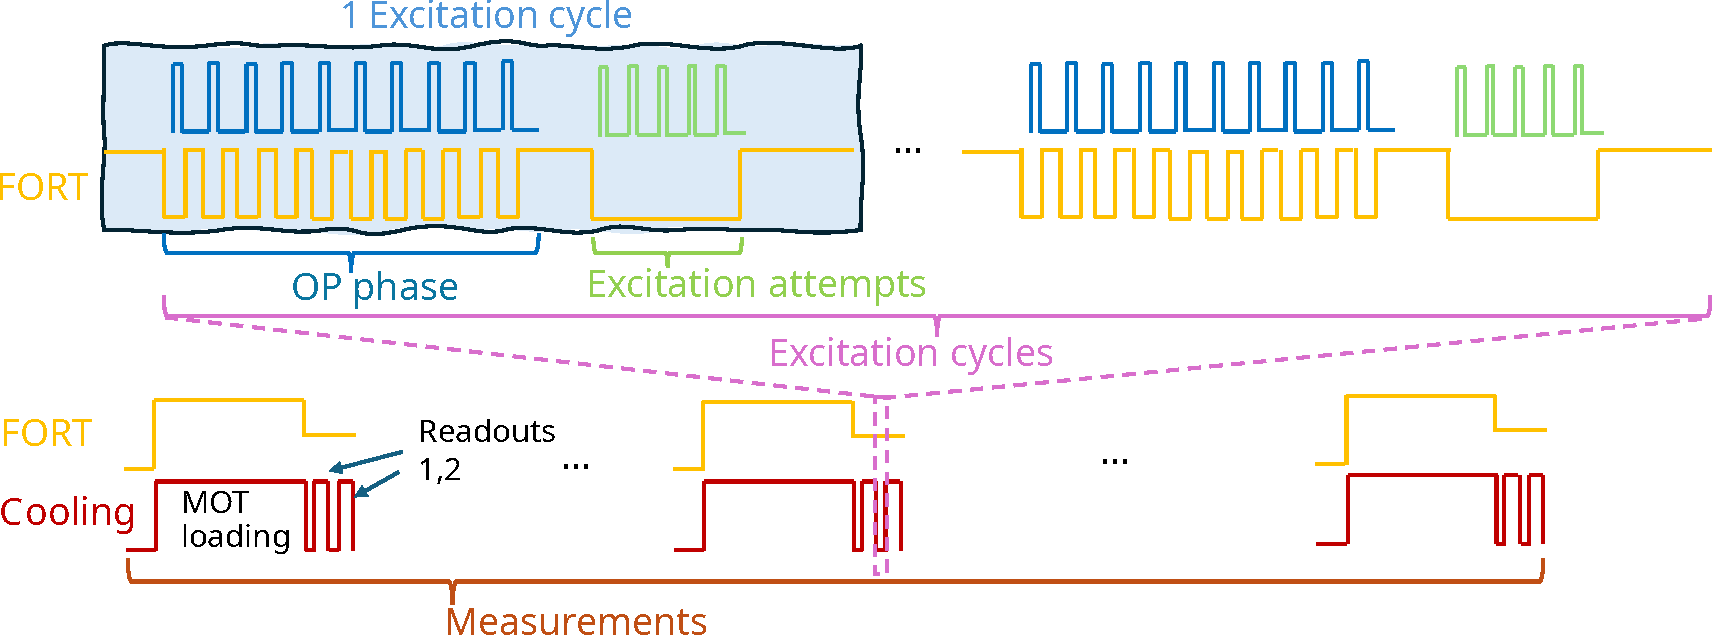
\includegraphics[width=\textwidth]{Images/single_photon_experiment_sequence.pdf}
    \caption{The experiment sequence loop for generating single photons, involving multiple sequences of chopped optical pumping (blue) and excitation attempts (green) per atom loaded. The nomenclature shown is used for consistency with what is used in the lab.}
    \label{fig:single_photon_sequence}
\end{figure}

The experiment sequence loop for generating single photons is shown in Fig. \ref{fig:single_photon_sequence}. For each atom loading attempt, multiple excitation cycles, defined as optically pumping the atom into $\ket{F=1,m_F=0}$ followed by at least one excitation pulse, are done in series several times. The exact number is chosen based on how likely the atom is to survive at the end of several cycles. The atom retention versus number of excitation cycles and the retention for 10 excitation cycles with varying amounts of recooling per cycle are shown in Fig. \ref{fig:sequence_survival_probability}. For the reported data, the recooling stages consists of turning on the MOT beams for some duration following the atom excitation, with the beam power and detuning used for the MOT, i.e., $2.5 \Gamma$ detuned from the bare $F=2\leftrightarrow F'=3$ cycling transition, or closer to $6 \Gamma$ including the AC Stark shifts from the FORT. It may be possible to acheive better cooling by going to lower power and more detuning. A limiting factor in this, however, is the extent to which the powers of opposing cooling beams are balanced and the magnetic field at the atom is near 0 (see Appendix \ref{ch:tempopt}). For now, the bias field of $\sim~3.2 $ G is left on continuously for the duration of the excitation loop.

\begin{figure}[!h]
    \centering
    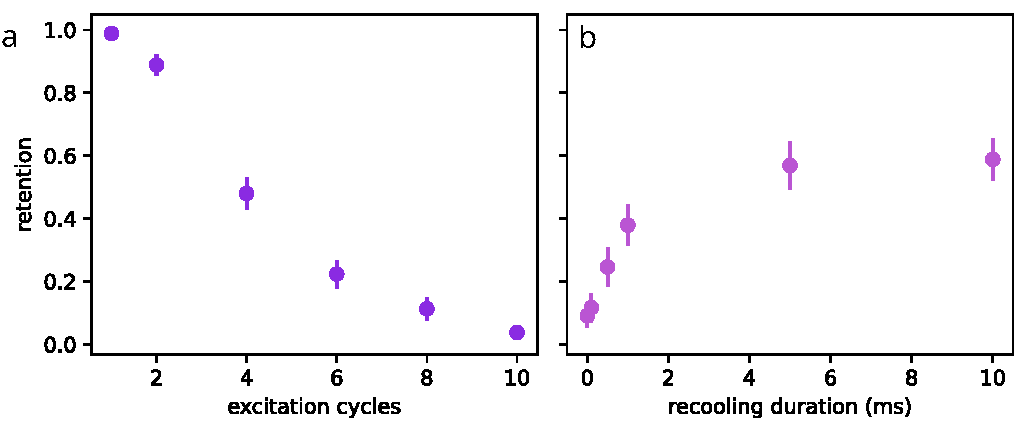
\includegraphics[width=\textwidth]{Images/retention_vs_excitation_cycles_and_recooling.pdf}
    \caption{(a) The probability an atom is retained following some number of excitation cycles with no recooling and (b) the probability of atom survival after 10 excitation cycles versus the duration of a recooling cycling appended to the end of each excitation cycle. For this data, there is only one excitation attempt per excitation cycle.}
    \label{fig:sequence_survival_probability}
\end{figure}

Note that multiple excitation pulses in series may be used without worry of more than one photon collected per series of excitation pulses, as the atom either decays into the $F=1$ stretched states which are dark to the excitation light, or it decays back to the inital state, the emission of which is $\pi$-polarized so we do not collect it (if the bias field is tuned correctly to be along the axis of the collection optics). Using several excitation pulses this way allows us to fight the per-pulse probability of $2/3$ to get $\sigma$-polarized emission and get probability approaching 1 after several attempts. Since the optical pumping takes an order of magnitude longer than the excitation pulse, even in the best case, it is advantageous to have multiple excitation pulses in series. 

\section{Photon extraction rate}
The photon extraction rate depends on both the per-attempt collection efficiency of our setup and the repetition rate with which we excite the atom. The 0.61 NA parabolic mirror can couple $\sigma$-polarized emission, which we get two-thirds of the time, from an atom trapped at the focus to an SM fiber with 0.12 efficiency in an ideal situation, i.e. where imperfections in the fiber coupling lens are neglected. In addition, there is finite loss through the dichroic that separates the $780 $nm photons from the FORT light path and loss through the bandpass filters before the detectors. Finally, there is finite coupling into MM fibers that go to the two SPCMs used for collection, each of which have around 0.65 quantum efficiency at 780 nm. The efficiencies of each step in the pipeline are summarized in Table \ref{table:collection_efficiency}.

\begin{table}[!h]
    \centering
    \begin{tabular}{ | m{2.2cm}| m{1cm} | }
        \hline
        Efficiency & Value \\
        \hline
        $\eta_{\sigma}$& 2/3 \\ 
        \hline
        $\eta_{\mathrm{mirror-to-fiber}} $& 0.12 \\
        \hline
        $\eta_{\mathrm{filters}} $& 0.94\footnotemark{} \\
        \hline
        $\eta_{\mathrm{MM}} $& 0.98 \\
        \hline
        $\eta_{\mathrm{SPCM}} $& 0.65 \\
        \hline
        $\eta_{\mathrm{total}} $& 0.044 \\
        \hline
    \end{tabular}
    \caption{Efficiencies through various elements in the path from atom to SPCMs.}
    \label{table:collection_efficiency}
\end{table}
\footnotetext{This is an approximation based on the comment by Akbar Safari that the two bandpass filters per SPCM and dichroic each had transmission over $98\%$.}

The repetition rate for generating photons once an atom is loaded depends primarily on the duration of time needed to optically pump the atom into $\ket{F=1,m_F=0}$ before each $\pi$ pulse. For the data presented in this thesis, the OP stage has not yet been optimized and therefore consumes typically 3 ms. The excitation pulse and collection window contribute a negligible amount of time by comparison, taking only $\sim~100$ ns. However, the OP time can be shortened to only a few $\mu \mathrm{s}$, perhaps at the expense of fidelity\cite{zhou2024long}. This would enable a peak photon detection rate on the order of $10^{5}~\mathrm{s}^{-1}$. Note however that this does not take into account recooling stages, and the average rate will be determined by how many times we need to reload an atom, which takes $\sim~500~\mathrm{ms}$ (see also Sec. \ref{sec:entanglementrate}).

\section{Excitation $\pi$-pulse}
As the lifetime of the $5P_{3/2}$ states is only 27 ns, we would like to excite the atom in less time than this to mitigate decay during the excitation, as this can lead to an effective jitter in the arrival time of photons due to decay during the excitation. Short pulses are broader in frequency and can potentially lead to unwanted excitation. The nearest state that could be excited off-resonantly is $\ket{5P_{3/2},F=2,m_F=0}$, which is nearly 230 MHz away (note that the $\ket{5S_{1/2},F=1,m_F=0} \leftrightarrow \ket{5P_{3/2},F=1,m_F=0}$ transition is electric dipole forbidden because $F$ and $m_F$ do not change). Thus for a pulse of width $\sim$10 ns, we can safely neglect off-resonant driving.

The excitation light, pulsed by an AOM, can be approximated by a Gaussian pulse in order to estimate how much power we need at the atoms for a given pulse width. The requirement to complete full population transfer with a time-varying Rabi frequency is 
\begin{equation}
\int_{t_1}^{t_2} \Omega(t') dt' =\pi
\end{equation}
For $\Omega(t)=\Omega_0 \exp({-\frac{t^2}{2\tau^2}})$, taking $t_1=-\infty$, and $t_2=\infty$ (most of the pule area is contained in a much shorter duration but this allows for a clean analytical result) and we have
\begin{equation} \label{eq:pi}
\begin{split}
\pi & = \Omega_0 \tau \sqrt{2 \pi} \\
 & = \Omega_0 \sqrt{2 \pi} \frac{t_{\textrm{FWHM}}}{2\sqrt{2\ln(2)}} \\
 & = \Omega_0 \sqrt{\pi} \frac{t_{\textrm{FWHM}}}{2\sqrt{\ln(2)}} \\
\end{split}
\end{equation}
which gives
\begin{equation}
    \Omega_0=\frac{2\sqrt{\pi \ln(2)}}{t_{\textrm{FWHM}}}
\end{equation}

% $\pi = \Omega_0 \tau \sqrt{2 \pi}$
% $= \Omega_0 \sqrt{2 \pi} \frac{t_{\textrm{FWHM}}}{2\sqrt{2\ln(2)}}$
% $= \Omega_0 \sqrt{\pi} \frac{t_{\textrm{FWHM}}}{2\sqrt{\ln(2)}}$
% $\Omega_0=\frac{2\sqrt{\pi \ln(2)}}{t_{\textrm{FWHM}}}$

Now we can calculate the power required to have $\Omega_0$ given a beam with a Gaussian spatial intensity pattern with $1/e^2$ waist $w_0$. 
\begin{equation}
    \Omega_0=\frac{dE}{\hbar}
\end{equation}
\begin{equation}
    I_0=\frac{2P_0}{\pi w_0^2}=\frac{1}{2}c \epsilon_0|E|^2
\end{equation}
\begin{equation}
    \Omega_0 =\frac{d}{\hbar}\sqrt{\frac{2I_0}
{c\epsilon_0}}=\frac{d}{\hbar}\sqrt{\frac{4P_0}{c\epsilon_0 \pi w_0^2}}
\end{equation}

Solving for $P_0$ gives
\begin{equation}\label{eq:p0}
\begin{split}
P_0 & = \frac{\hbar^2}{4d^2}\Omega_0^2\pi w_0^2 c \epsilon_0 \\
 & = \frac{\hbar^2}{4d^2} \pi w_0^2 c \epsilon_0 \left(\frac{2\sqrt{\pi \ln(2)}}{t_{\textrm{FWHM}}}\right)^2 \\
 & = \frac{\hbar^2}{d^2} \pi^2 w_0^2 c \epsilon_0\frac{\ln(2)}{t_{\textrm{FWHM}}^2} \\
\end{split}
\end{equation}
resulting in the peak Rabi frequency
\begin{equation}\label{eq:omega0}
    \Omega_0=\frac{2\sqrt{\pi \ln(2)}}{t_{\textrm{FWHM}}}.
\end{equation}
It can be shown with dimensional analysis that the units of Eq. \ref{eq:p0} are in fact power\footnote{Left as an exercise for the younger grad students.}.

The electric dipole matrix element for a transition $F,m_F$ to $F',m_F'$ on the $^{87}\textrm {Rb}$  $D_2$ line is given by
\begin{equation}d=4.227 e a_0 (-1)^{F'+J+1+I} \sqrt{(2 F'+1)(2 J+1)}\left\{\begin{array}{ccc}
J & J' & 1 \\
F' & F & I
\end{array}\right\}C_{F,m_F;1,-q}^{F',m_F'}
\end{equation}
where $\left\{ \begin{array}{c} \dots \\ \dots \end{array} \right\}$ is a Wigner $6j$ symbol, with $J=1/2$, $J'=3/2$, and $I=3/2$. The numerical prefactor times $e a_0$ is the fine structure reduced matrix element. Note that I use the convention $q = m_F' - m_F$, which opposite of what is used by others, e.g. Steck.
For $F=1, m_F=0$,  $F'=0, m_F'=0$, and linear polarization ($q=0$), we get
$|d|=5.636*10^{-30} ~\textrm{C}\cdot\textrm{m}$.
Now, we can evaluate what peak power we need to drive the $\pi$ rotation. The beam waist from either GRIN lens is about 300 $\mu \textrm{m}$. We can solve for the power with the relations above to get
\begin{equation}
    P_0 = c \epsilon_0 \pi^2 w_0^2 \frac{\hbar^2 \ln(2)}{d^2 t_{\textrm{FWHM}}^2}
\end{equation}
Using $t_{\textrm{FWHM}}=20~ \textrm{ns}$, we find $P_0 = 212~\mu \textrm{W}$.

As a sanity check, we can compare with a square pulse, for which the Rabi frequency needed is simply
\begin{equation}
    \Omega = \frac{\pi}{t}
\end{equation}
where $t$ is the pulse length. From the derivation above, we see \begin{equation}
    \frac{\Omega_{\textrm{square}}}{\Omega_{\textrm{Gaussian}}}=\frac{1}{2}\sqrt{\frac{\pi}{\ln(2)}} \approx 1.06
\end{equation}
The Rabi frequency scales as the square root of the power, so we have
\begin{equation}
\frac{P_{\textrm{square}}}{P_{\textrm{Gaussian}}} \approx 1.12
\end{equation}
Evidently, one needs about $10\%$ more power to excite the atom with a Gaussian pulse of the same nominal temporal length.

\section{Measuring $g^{(2)}$}

\subsection{The second-order quantum correlation function}
The test of whether the emission of our atoms is composed of single photon, that is, $\ket{n=1}$ Fock states, is measurement of the second-order quantum correlation function $g^{(2)}$. This correlation function, sometimes referred to as an intensity correlation, is given by\cite{gerry2004introductory}
\begin{equation}\label{eq:g2long}
    g^{(2)}(\tau) = \frac{\langle \hat{E}^{(-)}(t) \hat{E}^{(-)}(t+\tau) \hat{E}^{(+)}(t+\tau) \hat{E}^{(+)}(t) \rangle}{\langle \hat{E}^{(-)}(t) \hat{E}^{(+)}(t) \rangle \langle \hat{E}^{(-)}(t+\tau) \hat{E}^{(+)}(t+\tau) \rangle}.
\end{equation}
The positive frequency field operator $E^{(+)}$ at position $x$ for a single mode plane wave with angular frequency $\omega$ and wavevector $\mathbf{k}$ and mode volume $V$, is given by
\begin{equation}\label{eq:Epositive}
    \hat{E}^{(+)}(x) = i \left(\frac{\hbar \omega}{2 \epsilon_0 V}\right)^{\frac{1}{2}} \hat{a} e^{i(\mathbf{k\cdot r} - \omega t)}.
\end{equation}
and $\hat{a}$ is the annihilation operator. Evaluating Eq. (\label{eq:g2long}) for a single mode field thus reduces to
\begin{equation}\label{g2singlemode}
    g^{(2)}(\tau) = \frac{\langle \hat{a}^{\dagger}\hat{a}^{\dagger}\hat{a}\hat{a} \rangle}{\langle \hat{a}^{\dagger}\hat{a} \rangle}^2 = 1 + \frac{\langle (\Delta \hat{n})^2 \rangle - \langle \hat{n} \rangle}{\langle \hat{n} \rangle^2}
\end{equation}
which is independent of the delay time $\tau$. For a Fock state $\ket{n}$, this further reduces to 
\begin{equation}\label{eq:g2fock}
    g^{(2)}(\tau) = 1 - \frac{1}{n}
\end{equation}
which is less than 1 for all $n$, a signature that Fock states are non-classical. Of particular interest to the present work, single photon states result in $g^{(2)}(\tau)=0$. Note that $g^{(2)}$ is independent of $\tau$ for single-mode states, whereas, for example, a multi-mode field consisting of single photons in travelling modes spread out in time by $\Delta t$ would have $g^{(2)}(\tau) < g^{(2)}(0)$. This is an example of antibunching, which can be observed in atomic fluorescence\cite{schubert1992photon,volz2007atom}, since a single quantum emitter can not emit more than one photon simultaneously.

\subsection{Hanbury Brown Twiss measurement}

Intensity correlation measurements were first conducted by Hanbury Brown and Twiss for improving the baseline angular resolution of radio telescopes\cite{HANBURYBROWN1956} and later extended to measuring coherence in visible light\cite{brown1958interferometry}. Today, variations of their method is widely used in quantum optics for measuring $g^{(2)}$. The optical setup is relatively simple, consisting of a beamsplitter used to split a state of light incident on one port of the beamsplitter between two detectors at the output ports, shown in Fig. \ref{fig:hbtsetup}. By measuring the correlation of the intensity of a single mode field at the two detectors, one enacts a measurement of Eq. (\ref{eq:g2singlemode}).

\begin{figure}[!h]
    \centering
    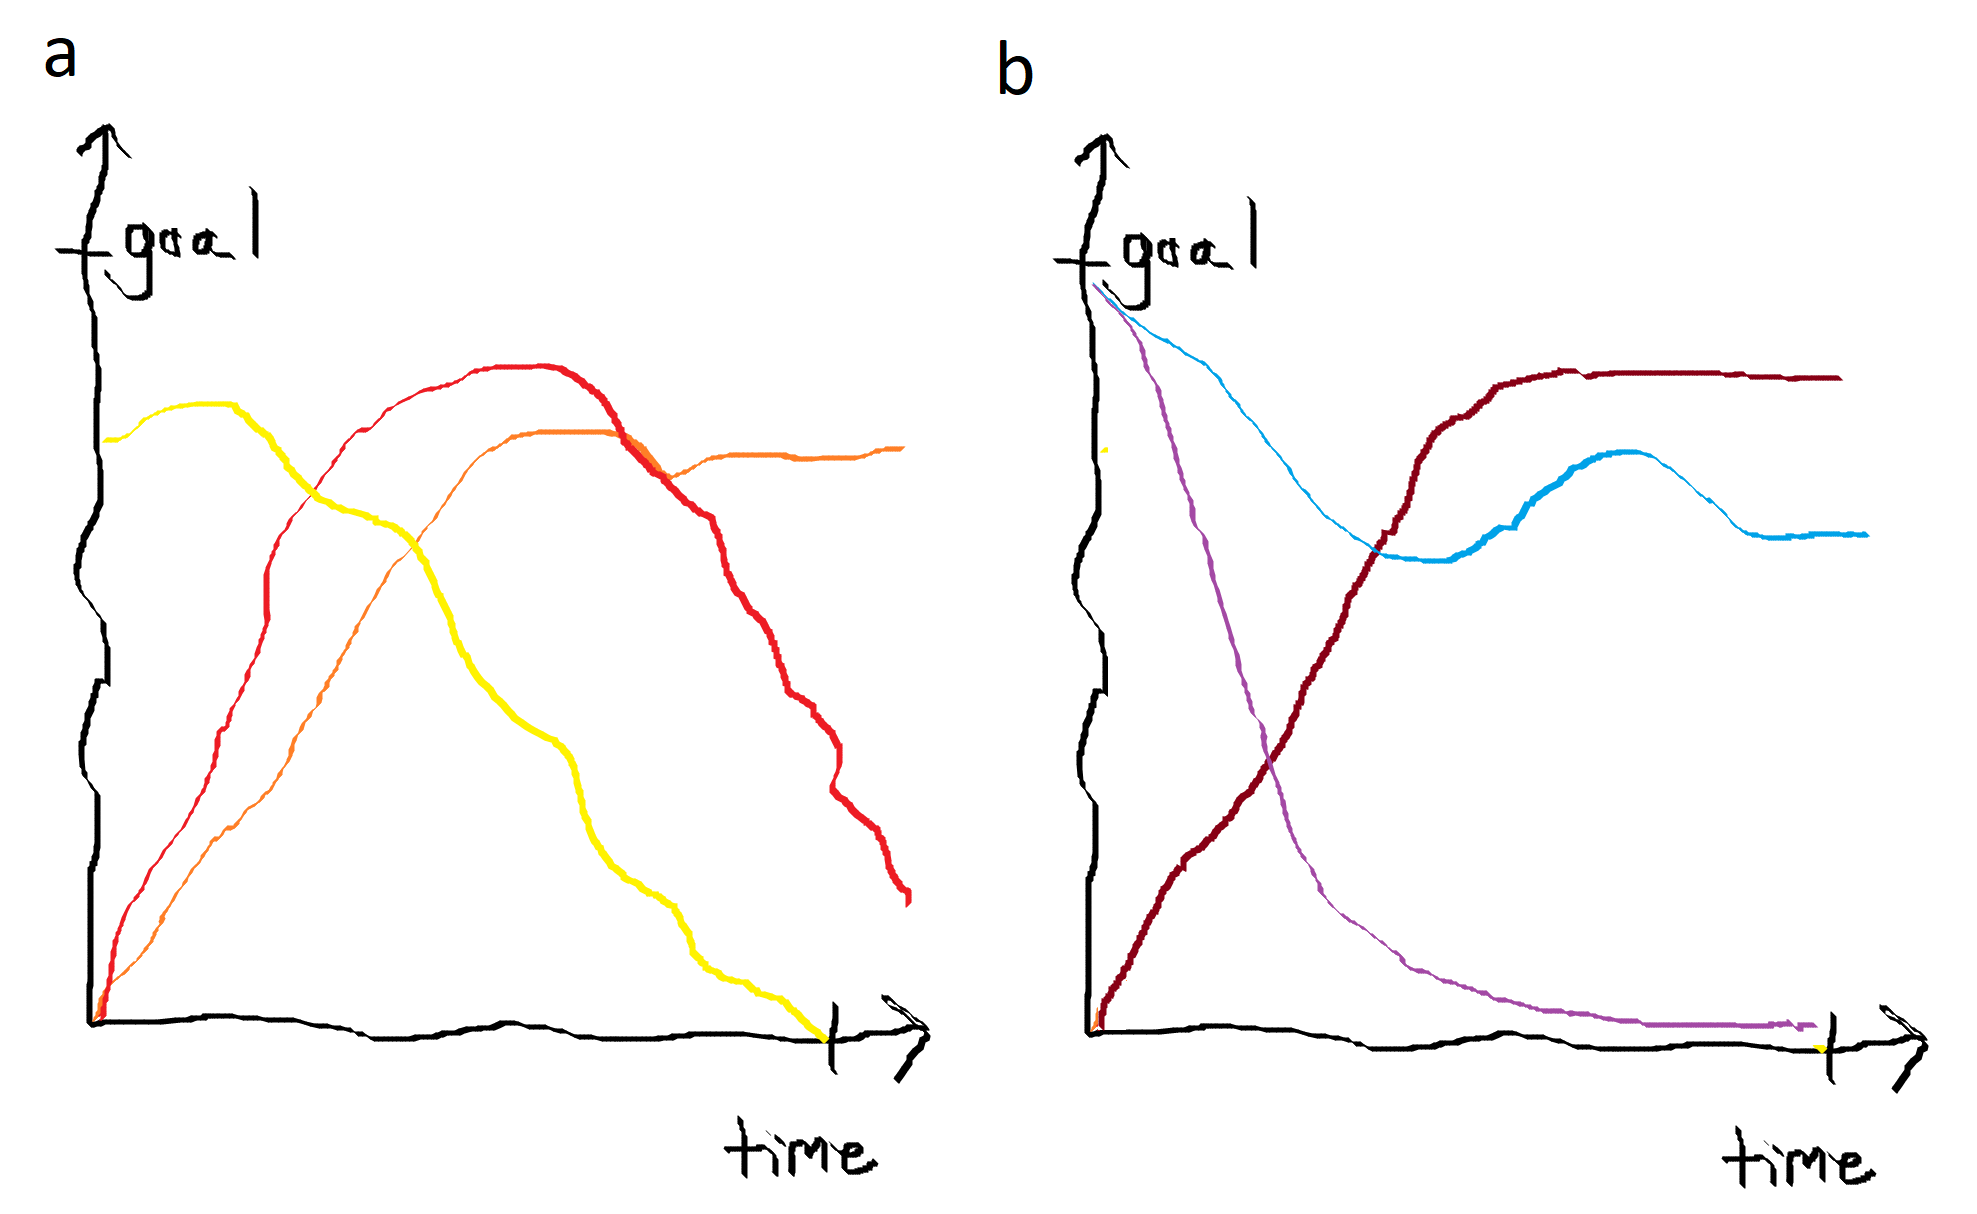
\includegraphics[width=\textwidth]{Images/fig_coming_soon.png}
    \caption{The optical setup for conducting a Hanbury Brown Twiss measurement.}
    \label{fig:hbtsetup}
\end{figure}

A non-polarizing beamsplitter can be described as a quantum operator which transforms the annihilation (or creation) operators at the input ports to those at the output ports according to
\begin{equation}
\left(\begin{array}{l}
    a_{c} \\
    a_{d}
    \end{array}\right)=\left(\begin{array}{ll}
    t^{\prime} & r \\
    r^{\prime} & t
    \end{array}\right)\left(\begin{array}{l}
    a_{a} \\
    a_{b}
\end{array}\right)
\end{equation}
where we will take $t=1/\sqrt{2}$ and $r=i/\sqrt{2}$. This results in 
\begin{equation}
\begin{aligned}
&a_{c}=\frac{1}{\sqrt{2}}\left(a_{a}+i a_{b}\right) \\
&a_{d}=\frac{1}{\sqrt{2}}\left(i a_{a}+a_{b}\right)
\end{aligned}
\end{equation}
which can be used, for example, to derive the famous Hong-Ou-Mandel effect\cite{Hong1987}.

% It is clear that for an input state $\ket{0}_a+\ket{0}_b$





